\subsection{Materia necesaria}

\begin{definicion}{Cartas \(\bar X\)-R}
Cuando cada observacion es una submuestra pequena, se controla simultaneamente el promedio y la dispersion. La carta \(\bar X\) detecta desplazamiento del centro; la carta R detecta exceso de variabilidad.
\end{definicion}

\begin{formulas}{Constantes para \(n=4\)}
Para submuestras de tamano \(n=4\):
\[
A_2=0.729,\qquad D_3=0,\qquad D_4=2.282.
\]
\[
LCS_{\bar X}=\bar{\bar X}+A_2\bar R,\quad
LCI_{\bar X}=\bar{\bar X}-A_2\bar R,
\]
\[
LCS_R=D_4\bar R,\quad LCI_R=D_3\bar R.
\]
\end{formulas}

\begin{definicion}{Muestreo de aceptacion}
El muestreo de aceptacion se usa cuando se reciben lotes de un proveedor y no se quiere inspeccionar el \(100\%\) de las unidades. En vez de revisar todo el lote, se toma una muestra aleatoria de \(n\) unidades y se cuenta cuantas vienen defectuosas. Un plan de muestreo simple se escribe como:
\[
(n,c),
\]
donde \(n\) es el tamano de muestra y \(c\) es el numero maximo de defectuosas permitido para aceptar el lote. Si \(d\) es el numero de defectuosas observadas en la muestra, la regla es:
\[
\text{aceptar el lote si }d\le c,
\qquad
\text{rechazar el lote si }d>c.
\]
\end{definicion}

\begin{definicion}{AQL, LTPD, \(\alpha\) y \(\beta\)}
Los cuatro parametros se leen asi:
\[
\begin{array}{lll}
AQL & \text{calidad buena} & \text{fraccion defectuosa aceptable},\\
LTPD\ \text{o}\ LPTD & \text{calidad mala} & \text{fraccion defectuosa rechazable},\\
\alpha & \text{riesgo del productor} & \text{rechazar un lote bueno},\\
\beta & \text{riesgo del consumidor} & \text{aceptar un lote malo}.
\end{array}
\]
Por eso un plan debe aceptar con alta probabilidad cuando \(p=AQL\), y aceptar con baja probabilidad cuando \(p=LTPD\).
\end{definicion}

\begin{definicion}{Errores tipo I y tipo II en muestreo}
Si se mira como una decision estadistica, aceptar o rechazar un lote tiene dos errores posibles:
\[
\begin{array}{lll}
\text{Error tipo I} & =\alpha & \text{rechazar un lote bueno, con }p=AQL,\\
\text{Error tipo II} & =\beta & \text{aceptar un lote malo, con }p=LTPD.
\end{array}
\]
En palabras simples, \(\alpha\) protege al productor o proveedor, porque evita rechazar lotes que tienen calidad aceptable. En cambio, \(\beta\) protege al consumidor o comprador, porque evita aceptar lotes de mala calidad.
\end{definicion}

\begin{formulas}{Curva OC de un plan \((n,c)\)}
Si \(p\) es la fraccion defectuosa real del lote, y se aproxima el numero de defectuosas en la muestra por una binomial,
\[
D\sim \operatorname{Binomial}(n,p),
\]
entonces la probabilidad de aceptar el lote es:
\[
P_a(p)=P(D\le c)
=\sum_{d=0}^{c}\binom{n}{d}p^d(1-p)^{n-d}.
\]
Para que el plan cumpla las condiciones del enunciado debe satisfacer:
\[
P_a(0.02)\ge 0.95,
\qquad
P_a(0.08)\le 0.10.
\]
Intuitivamente, el plan debe aceptar casi siempre cuando el proveedor entrega buena calidad, pero debe rechazar casi siempre cuando entrega mala calidad.
\end{formulas}

\begin{center}
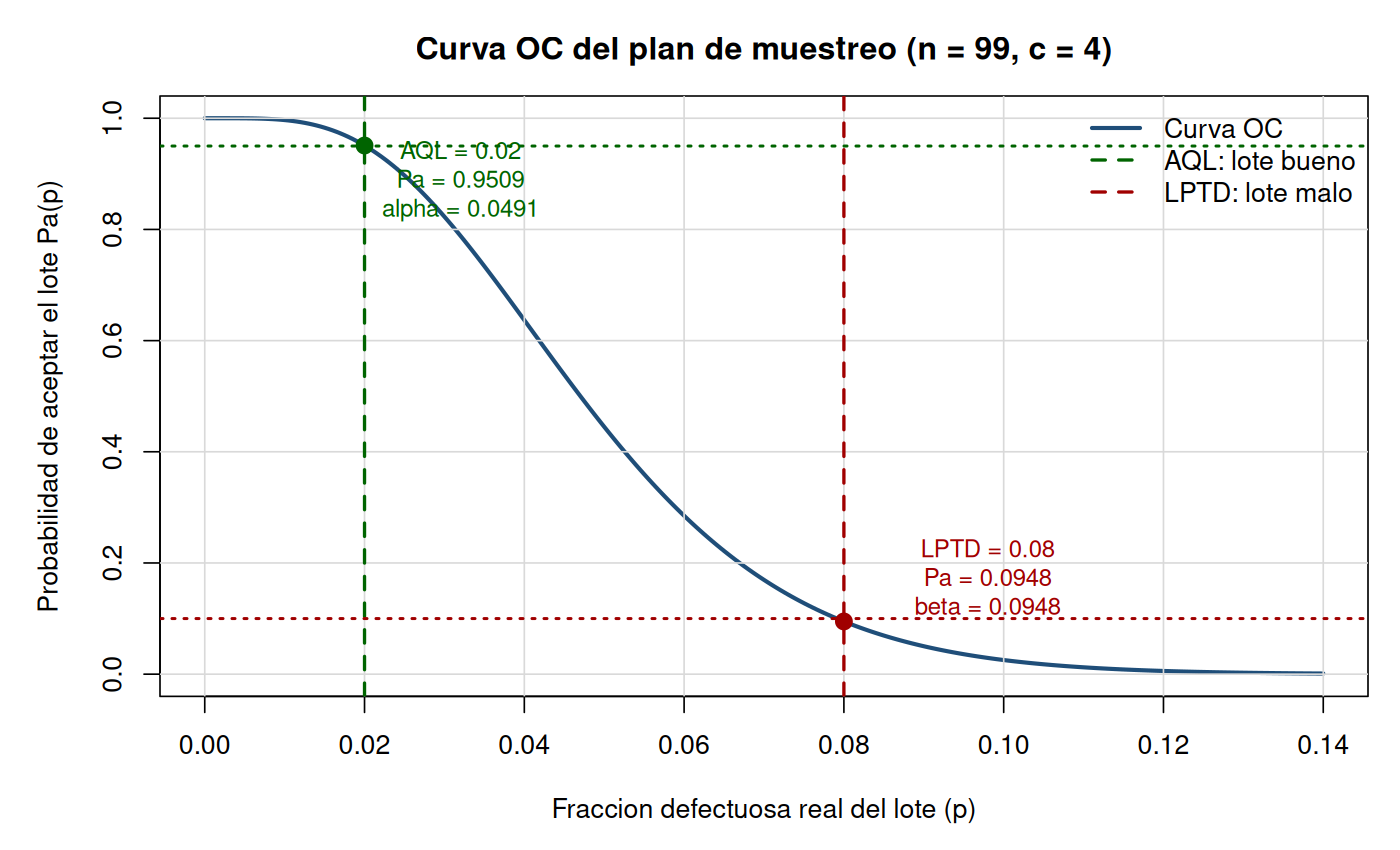
\includegraphics[width=0.88\textwidth]{ejercicios/03/figuras/curva_oc_muestreo.png}
\end{center}

\begin{trampa}{Como leer la curva OC}
La curva OC baja cuando aumenta la fraccion defectuosa \(p\). En \(p=AQL=0.02\), se quiere \(P_a(p)\) alto: ahi \(1-P_a(AQL)=\alpha\). En \(p=LTPD=0.08\), se quiere \(P_a(p)\) bajo: ahi \(P_a(LTPD)=\beta\). Por eso no basta elegir \(n\) grande; el par \((n,c)\) debe equilibrar ambos riesgos.
\end{trampa}

\begin{trampa}{Lectura rapida del problema}
El \(AQL\) no es el porcentaje que se acepta en la muestra; es la calidad considerada buena del lote completo. El \(LTPD\) tampoco es el porcentaje observado en la muestra; es la calidad considerada mala del lote completo. El numero \(c\) se elige para que el plan tenga las probabilidades de aceptacion deseadas en esos dos puntos de calidad.
\end{trampa}
